\documentclass[12pt]{article}

\usepackage{answers}
\usepackage{setspace}
\usepackage{graphicx}
\usepackage{enumitem}
\usepackage{multicol}
\usepackage{mathrsfs}
\usepackage[margin=1in]{geometry} 
\usepackage{amsmath,amsthm,amssymb}
 
\newcommand{\N}{\mathbb{N}}
\newcommand{\Z}{\mathbb{Z}}
\newcommand{\C}{\mathbb{C}}
\newcommand{\R}{\mathbb{R}}

\DeclareMathOperator{\sech}{sech}
\DeclareMathOperator{\csch}{csch}
 
\newenvironment{theorem}[2][Theorem]{\begin{trivlist}
\item[\hskip \labelsep {\bfseries #1}\hskip \labelsep {\bfseries #2.}]}{\end{trivlist}}
\newenvironment{definition}[2][Definition]{\begin{trivlist}
\item[\hskip \labelsep {\bfseries #1}\hskip \labelsep {\bfseries #2.}]}{\end{trivlist}}
\newenvironment{proposition}[2][Proposition]{\begin{trivlist}
\item[\hskip \labelsep {\bfseries #1}\hskip \labelsep {\bfseries #2.}]}{\end{trivlist}}
\newenvironment{lemma}[2][Lemma]{\begin{trivlist}
\item[\hskip \labelsep {\bfseries #1}\hskip \labelsep {\bfseries #2.}]}{\end{trivlist}}
\newenvironment{exercise}[2][Exercise]{\begin{trivlist}
\item[\hskip \labelsep {\bfseries #1}\hskip \labelsep {\bfseries #2.}]}{\end{trivlist}}
\newenvironment{solution}[2][Solution]{\begin{trivlist}
\item[\hskip \labelsep {\bfseries #1}]}{\end{trivlist}}
\newenvironment{problem}[2][Problem]{\begin{trivlist}
\item[\hskip \labelsep {\bfseries #1}\hskip \labelsep {\bfseries #2.}]}{\end{trivlist}}
\newenvironment{question}[2][Question]{\begin{trivlist}
\item[\hskip \labelsep {\bfseries #1}\hskip \labelsep {\bfseries #2.}]}{\end{trivlist}}
\newenvironment{corollary}[2][Corollary]{\begin{trivlist}
\item[\hskip \labelsep {\bfseries #1}\hskip \labelsep {\bfseries #2.}]}{\end{trivlist}}
 
\begin{document}
 
% --------------------------------------------------------------
%                         Start here
% --------------------------------------------------------------
 
\title{FINAL Study Guide}%replace with the appropriate homework number
\author{Andrew Reed\\ %replace with your name
Course-Semester} %if necessary, replace with your course title
 
\maketitle

\tableofcontents

\pagebreak

\section{Trigonometry}

\subsection{Basic Trigonometry}
\[
	sin(x) = \left [ \frac{Opposite}{Hypotenuse} \right ] \rightarrow csc(x) = \frac{1}{sin(x)}
\]
\[
	cos(x) = \left [ \frac{Adjacent}{Hypotenuse} \right ]  \rightarrow sec(x) = \frac{1}{cos(x)}
\]
\[
	tan(x)= \left [ \frac{Opposite}{Adjacent} \right ] \rightarrow cot(x) = \frac{1}{tan(x)}
\]

\subsection{Trigonometry Derivatives}
\[
	\frac{d}{dx} sin(x) = cos(x) \quad \quad \quad \frac{d}{dx} csc(x) = -cot(x)csc(x)
\]
\[
	\frac{d}{dx} cos(x) = -sin(x) \quad \quad \quad \frac{d}{dx} sec(x) = sec(x)tan(x)
\]
\[
	\frac{d}{dx} tan(x) = sec^{2}(x) \quad \quad \quad \frac{d}{dx} cot(x) = -csc^{2}(x)
\]

\subsection{Inverse Trigonometry Derivatives}
\[
	\frac{d}{dx}sin^{-1}(x) = \frac{1}{\sqrt{1-x^{2}}} \quad \quad \quad \frac{d}{dx}cos^{-1}(x) = - \frac{1}{\sqrt{1-x^{2}}}
\]
\[
	\frac{d}{dx}tan^{-1}(x) = \frac{1}{1 + x^{2}} \quad \quad \quad \frac{d}{dx}cot^{-1}(x) = - \frac{1}{1 + x^{2}}
\]
\[
	\frac{d}{dx}sec^{-1}(x) = \frac{1}{\left | x \right | \sqrt{x^{2} - 1}} \quad \quad \quad \frac{d}{dx}csc^{-1}(x) = - \frac{1}{\left | x \right | \sqrt{x^{2} - 1}} 
\]
\pagebreak


\section{Integral}

\subsection{Table of Integrals}
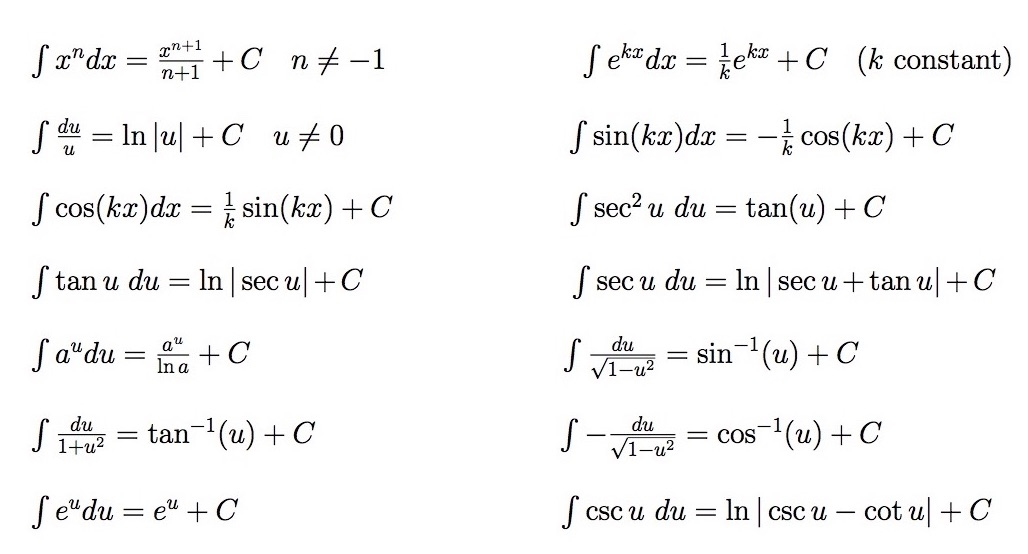
\includegraphics[width=\linewidth]{IntegralTable}


\subsection{Mean Value Theorem ( Average Value Theorem ) }
\[
	\frac{1}{a-b} \int_a^b f(x) dx = f(c)
\]

\subsection{Area Under A Curve}
\[
	\int_a^b f(x) dx
\]

\subsection{Area Between Two Curves}


\[
	\int_a^b \left [ f(x) - g(x) \right ] dx
\]


\subsection{Integration by Parts}
\[
	\int u dv = u v - \int v du
\]

\subsection{Partial Fractions}
\[
	\frac{p(x)}{(x - a)(x-b)} = \frac{A}{x-a} + \frac{B}{x-b}
\]
\[
	\frac{p(x)}{(x - a)^{2}} = \frac{A}{x-a} + \frac{B}{(x-a)^{2}}
\]

\subsection{Simpson's Rule}
\[
	\int_a^b f(x) dx \approx S_n
\]
\[
	S_n = \frac{\Delta x}{3} \left [ f(x_0) + 4f(x_1) + 2f(x_2) + 4f(x_3) + ... + 2f(x_{n-2}) + 4f(x_{n-1}) + f(x_n) \right ]
\]
\[
	\Delta x = \frac{b - a}{n}
\]

\subsection{Improper Integrals}
\[
	\int_a^\infty f(x) dx = \lim_{n\rightarrow \infty} \int_a^n f(x) dx
\]
\[
	\int_\infty^b f(x) dx = \lim_{n\rightarrow \infty} \int_n^b f(x) dx
\]
\[
	\int_\infty^\infty f(x) dx = \lim_{n\rightarrow \infty} \int_n^b f(x) dx +  \lim_{n\rightarrow \infty} \int_n^b f(x) dx
\]


\subsection{Arc Length Formula}
\[
	L = \int_a^b \left ( \sqrt{1 + \left [ \frac{dy}{dx} \right ]^{2} } \right ) dx
\]



\section*{Volume}

\subsection{Disk Method}
\[
	V = \pi \int_a^b \left [ f(x) \right ] ^{2} dx
\]

\subsection{Washer Method}
\[
	V = \pi \int_a^b \left [ \left ( f(x) \right ) ^{2} - \left ( g(x) \right )^{2} \right ] dx
\]

\subsection{Shells Method}
\[
	V = 2 \pi \int_a^b \left [ x  f(x) \right ] dx
\]
\[
	V = 2 \pi \int_a^b  x  \left [ f(x) - g(x) \right ] dx
\]\pagebreak

\section{Polar Curves}

\subsection{Derivatives of Polar Curves}
\[
	\frac{dy}{dx} = \frac{ \frac{dy}{dt} }{ \frac{dx}{dt} } \quad If \frac{dx}{dt} \neq 0
\]

\subsection{Polar And Cartesian}

\[
	x = r cos(\theta) \quad And \quad y = r sin(\theta)
\]
\[
	r^{2} = x^{2} + y^{2}
\]
\[
	tan(\theta) = \frac{y}{x}
\]

\pagebreak


\section{Series}

\subsection{Order Of Operations}
\includegraphics[width=\linewidth]{Series_Diagram.png}


\subsection{Harmonic Series}

\begin{enumerate}
\item $\frac{1}{x}$ , is a harmonic Series and it Diverges
\end{enumerate}


\subsection{Test for Divergence}

\begin{enumerate}
\item If [ $\lim_{n\rightarrow \infty} a_n \neq 0$ ] is true then the series diverges
\end{enumerate}


\subsection{Alternating Series}

\begin{enumerate}
\item Confirm $\left( -1 \right) ^{n} $ exists
\item If [ $\lim_{n\rightarrow \infty} a_n = 0$ ] than the series Converges
\item If [ $\lim_{n\rightarrow \infty} a_n \neq 0$ ] than the series Diverges
\end{enumerate}


\subsection{Geometric Series}

\begin{enumerate}
\item For a series to be geometric it must have a value that is continuously added, such as a function $(c)^{n}$ where the series grows by a constant C each iteration.
\item If C $<$ 1 then the series converges
\item  If C $>$ 1 or C = 1 then the series diverges
\end{enumerate}


\subsection{P Series}

\begin{enumerate}
\item  Confirm $ \left [ \frac{1}{n^{p} } \right ]$ exists
\item If p $>$ 1 than the series converges
\item If p $<$ 1 or p = 1 than the series diverges
\end{enumerate}


\subsection{Integral Series}

\begin{enumerate}
\item  Set $a_n = f(x)$
\item Change $\sum\limits_{n=a}^{b} a_n$ To $\int_a^n f(x)$ 
\end{enumerate}


\subsection{Direct Comparison Test}

\begin{enumerate}
\item 0 $\leq a_n \leq  b_n$ 
\item If $\sum\limits_{n=a}^{b} b_n$ converges then, $\sum\limits_{n=a}^{b} a_n$  converges 
\item If $\sum\limits_{n=a}^{b} a_n$ diverges then, $\sum\limits_{n=a}^{b} a_n$  diverges 
\end{enumerate}


\subsection{Limit Comparison Test}

\begin{enumerate}
\item When you have the given series $\sum\limits_{n=a}^{b} a_n$ and what you believe looks like $\sum\limits_{n=a}^{b} b_n$  if $\lim_{n \rightarrow \infty } \frac{a_n}{b_n} $ exists than either both series converge or both series diverge.
\end{enumerate}


\subsection{Ratio Test}

\begin{enumerate}
\item $\rho = \lim_{n \rightarrow \infty} | \frac{a_{n+1}}{a_n} |$
\item If $\rho < 1$, the series converges absolutely
\item If $\rho > 1$, the series diverges
\item If $\rho = 1$, the series is unable to be determined still
\end{enumerate}


\subsection{Root Test}

\begin{enumerate}
\item If the series can be written as $ \left ( a_n \right ) ^{k}$ then root test is applicable.
\item $\rho = \lim_{n \rightarrow \infty}  |a_n| ^{ \frac{1}{k} }$
\item If $\rho < 1$, the series converges absolutely
\item If $\rho > 1$, the series diverges
\item If $\rho = 1$, the series is unable to be determined still
\end{enumerate}


\subsection{Telescoping Series}

\begin{enumerate}
\item Telescoping series are any series that can be written out as;
\[
	\lim_{n \rightarrow \infty}  a_n = (b_1 - b_2) + (b_2 - b_3) + (b_3 - b_4) + ...
\]
\item Almost every term should be canceled with its preceding term
\item Partial fractions is often used here
\item Partial sums is often recommended for these series
\end{enumerate}


\subsection{Power Series}

\begin{enumerate}
\item $a_n$ that is dominated by geometric growth
\item Most commonly seen as, $f(x) = \frac{a}{1-r}$
\end{enumerate}


\subsection{Radius of Convergence}

\begin{enumerate}
\item Put in terms of $( a_n )^{k}$
\item solve r = $|a_n| < 1$
\item Radius of Convergence = $(-r, r)$
\end{enumerate}


\subsection{Interval of Convergence}

\begin{enumerate}
\item If it is not obvious than using ratio test to find r is helpful.
\item $|r| < 1$
\item Put in terms of $(x - a) < b$ than the interval of convergence is $(b-a, b+a)$
\item If the point is convergent change ( or ) to [ or ]
\end{enumerate}


\end{document}
